\chapter{Neukonzeption}

\section{ADM als Methode}
Die Architecture Development Method (ADM) ist ein Vorgehensmodell, das den Kernbestandteil von TOGAF darstellt. 
Dieses iterative Verfahren dient zur Konzeption und Verwaltung von Geschäftsarchitekturen und besteht aus acht aufeinanderfolgenden Phasen, sowie einer projektvorbereitenden Phase.
Zentrales Element dieses Modells ist das Anforderungsmanagement.
Dieses sagt aus, dass sich die Schritte entlang des Zyklus immer wieder an den Anforderungen und geschäftlichen Zielen ausgerichtet werden, welche sich im Laufe eines Projekts z.B. durch geschaffene Möglichkeiten verändern können.\\
\begin{figure}[!htb]
\centering
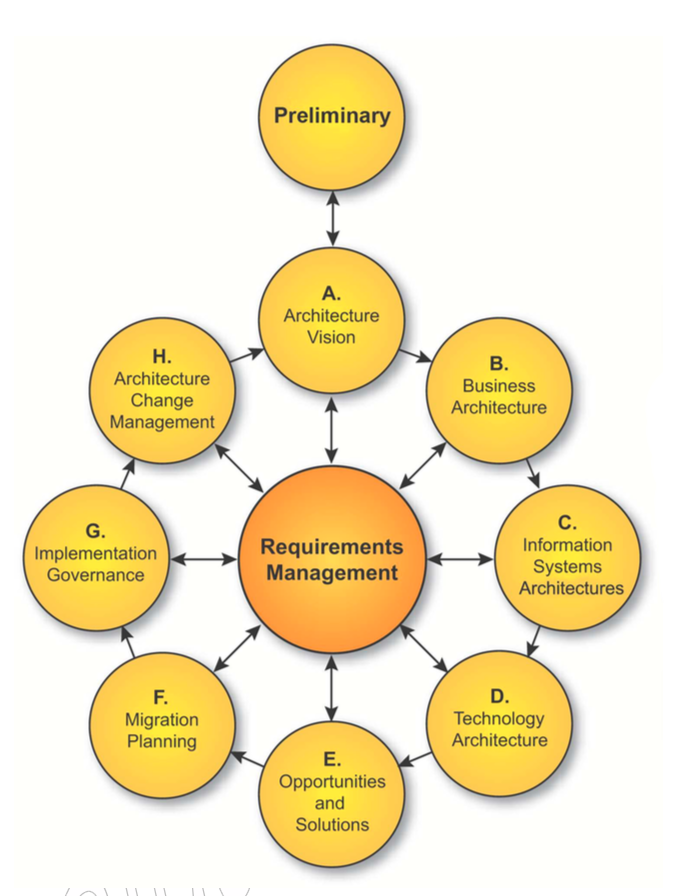
\includegraphics[height=80mm]{images/adm-cycle}
\caption[ADM-Zyklus]{Der ADM-Zyklus \protect\footnotemark}
\label{ADM-Zyklus}
\end{figure}
\footnotetext{Quelle: \cite{TOGAF} S.48 }
\\
Dabei gilt, dass jede Phase einen Output liefert, der als Input für die nächste Phase benutzt wird.\\
Aufgrund des Umfanges werden in dieser Arbeit die Phasen bis C betrachtet. Die konzeptionelle Arbeit wird bis Phase D geleistet, diese wird allerdings ausgeklammert.
\begin{enumerate}
\item{Preliminary}
\\ In der vorgelagerten Phase findet die Eingrenzung des Umfangs auf Basis der Anforderungen statt. 
Ein weiterer Bestandteil ist das ''Tailoring'' statt, in dem das methodische Vorgehen geplant und ggf. gegenüber dem Framework (TOGAF) angepasst wird.\\
Output ist das Dokument ''Request For Architecture Work'' (RFA), das Ausgangspunkt des Requirement Management ist.
\item{Phase A: Architecture Vision}
\\ In dieser Phase wird richtungsweisend definiert, auf welche Art die zu konzeptionierende Infrastruktur den Anforderungen und Zielen Rechnung tragen soll. Dabei wird auch auf Weiter- oder Wiederverwendungsmöglichkeiten von Bestandsressourcen geschaut.\\
Dies wird in das Dokument''Statement Of Architecture Work'' als Output überführt.
\item{Phase B: Business Architecture}
\\ Phase B definiert die Geschäftsarchitektur hinsichtlich Aufbau- und Ablauforganisation. Das bedeutet, dass hierbei die Anforderungen in konkrete Funktionen und Abläufe überführt werden, was den Output dieser Phase darstellt.
\item{Phase C: Information Systems Architectures}
\\ Die letzte betrachtete Phase definiert die logische Informationsarchitektur hinsichtlich Datenhaltung (Data Architecture) und -verarbeitung (Application Architecture). \\
Ein Datenhaltungsmodell und die erforderliche Anwendungs- und Schnittstellenlandschaft werden festgelegt.
\item{Phase D: Technology Architecture}
\\ Die letzte betrachtete Phase definiert die Architektur, die es der logischen und physische



\end{enumerate}


\section{Preliminary}
% erzeugt die parameter für eine erfolgreiche iteration in der adm
Den Einstieg in ein TOGAF-Projekt bildet die erste Phase im ADM-Zyklus, die den Titel Preliminary (dt. Vorbereitung, Einleitung) trägt und die generellen Rahmenparameter setzt und beschreibt.
Dazu gehört einerseits, den die Abgrenzung des Umfangs zu definieren, aber auch das Tailoring, das das methodische Vorgehen im weiteren Verlauf erläutert.

\subsection{Scope}
ADM wird in Verbindung mit dem gesamten Framework der Open Group in der Regel in großen Projekten eingesetzt und bietet die Möglichkeit, auch im Hinblick auf Arbeit mit Global Playern eingesetzt werden zu können.
Der in der Einleitung beschriebene Rahmen weicht maßgeblich von solchen Vorhaben ab.
Im Fokus steht der Workflow zur Bearbeitung eingehender Kreditorenrechnungen, der als End-To-End-Prozess zu verstehen ist.
Er beginnt mit einer eingehenden Rechnung und endet mit deren Bezahlung.
Zu betrachten ist zunächst der Ablauf dieses Prozesses und wie er an der Aufbauorganisation der \firma ausgerichtet ist, also seine Stakeholder und Akteure sowie deren Aktivitäten im Prozessverlauf.
Die Basis dieses Kontinuums bilden die Informationssystemarchitektur, die wiederum auf der technologischen Infrastruktur aufbaut, deren Bestand und im Rahmen struktureller Veränderungen notwendiger zukünftiger Umfang ebenfalls untersucht werden.
Die detaillierte Definition des Umfangs erfolgt in der nächsten Phase.

\subsection{Tailoring}
Das sogenannte Tailoring dient dazu, die von TOGAF vorgeschlagenen Schritte und Methoden dem Anforderungsportfolio des Projekts anzupassen.
Der in dieser Arbeit vorgestellte Rahmen ist deutlich weniger umfangreich als z.B. eine konzernweite Umstrukturierung einer großen Anwendungslandschaft, was zur Folge hat, dass die Verwendung der formalen Methoden auf diesen Zweck hin ausgerichtet werden muss.
Außerdem stehen im Zentrum von ADM-Iterationen in der Regel Dokumente wie der RFA, die über das Projekt versioniert und weitergegeben werden.
Das auf diese weise realisierte Requirements Management ist darauf ausgerichtet, die fortgeschriebenen Anforderungen immer wieder gemäß dem Fortschritt und den daraus resultierenden geplanten Veränderungen stets in den Fokus zu stellen und ergebnisorientierte Arbeit zu ermöglichen.
Da diese Arbeit lediglich von einem Autor angefertigt wird, ist eine teamübergreifende Kommunikation nicht notwendig.
Durch Versionierung von auf Kommunikation ausgelegten Dokumenten  zwangsläufig entstehende Redundanzen sollen demnach vermieden werden.
Das heißt, dass die Phasen des ADM-Zyklus (bzw. die drei konzeptionellen Phasen) gesondert betrachtet werden.
In diesen wird jeweils die bestehende Geschäftsarchitektur (Baseline Architecture) je nach Phase in einer bestimmten Hinsicht aufgenommen.
Danach wird eine in dieser Hinsicht verbesserte Geschäftsarchitektur konzipiert und in einer Analyse der Baseline Architecture gegenübergestellt. 
Diese Gap-Analysis stellt die bei der geplanten Transistion der Geschäftsarchitektur Bestandteile in einen Implementationskontext, welcher definiert, ob Bestandskomponenten in einer möglichen Art weiterverwendet oder gänzlich verworfen werden sollen, und ob Plankomponenten auf weiterverwendeten Komponenten basieren können oder neu entwickelt werden müssen.
In einem weiteren Analyseschritt wird evaluiert, welche Auswirkungen sich aus den geplanten Änderungen ergeben und wer bzw. was auf welche Art davon betroffen ist. 
Dieser Vorgang wird als Impact Assessment bezeichnet.


\section{Phase A: Architecture Vision}
Aufgabe der Phase A ist es, richtungsweisend zu definieren, welche Fähigkeiten von der zu konzeptionierenden Architektur abzudecken sind und welcher geschäftliche Mehrwert durch sie zur Verfügung gestellt werden soll.
Der zu nutzende Input ist das Dokument ''Request for Architecture Work'', welches zwar einerseits aus der Phase Preliminary hervorgeht, maßgeblich jedoch im parallel angefertigten Praxisbericht umschrieben wurde und die Problematik des Ist-Zustands darstellt, welche wiederum die inhaltliche Motivation der Prozesstreiber bedingt.
Die detaillierte Absteckung des Umfangs bildet die Ausgangslage für alle folgenden Schritte, auf Basis derer das Projekt mit dieser Phase etabliert werden soll.
Dazu erfolgt zunächst die Einordnung der identifizierten Stakeholder und ihrer Interessen.
Die Beschreibung des zu erzielenden Mehrwerts erfolgt nach Darlegung der zu beachtenden Richtlinien (in TOGAF Constraints bezeichnet).

\subsection{Scope}
Um den Umfang des durchzuführenden Projekts genau einordnen zu können, muss definiert werden, 
\begin{itemize}
\setlength\itemsep{-0.2em}
\item{welche Teile der Geschäftsarchitektur  im Fokus stehen und daher ausgewertet und bearbeitet werden,}
\item{welche Teile der Geschäftsarchitektur zwar im Kontext stehen, allerdings nicht betrachtet werden,}
\item{und welche Teile der Geschäftsarchitektur als optional betrachtet werden.}
\end{itemize}

Der Umfang wird durch mehrere Attribute beschrieben. 
In ihrer Gesamtheit ergeben diese Attribute den zu betrachtenden Rahmen des Projekts, der nötig ist, um erfolgreich den zu erbringenden Mehrwert in der Organisation etablieren zu können.

\subsubsection{Prozesse}
Der Umfang der betrachteten Prozesse ergibt sich aus der Themenstellung, wird aber der Vollständigkeit noch einmal erläutert.
Der zu betrachtende Prozess der Kreditorenrechnungsbearbeitung beginnt mit einem Rechnungseingang, verläuft über Freigaben bis zur Buchung und geht dann in die Zahlung, welche erneut freigegeben werden muss.
Alle damit im Zusammenhang stehenden Tätigkeiten, die zur vollständigen Abarbeitung und zur Erreichung des Ziels (bezahlte Kreditorenrechnung) sind damit Kern der Betrachtung, also:
\\[1\baselineskip]
Rechnungseingang $\rightarrow$ Sachliche Prüfung und Freigabe $\rightarrow$ Fachliche Prüfung und Freigabe $\rightarrow$ Rechnungsbuchung $\rightarrow$ Zahllauferstellung $\rightarrow$ Zahllauffreigabe $\rightarrow$ Zahlung
\\[1\baselineskip]
Periphere Anforderungen wie eine rückwirkende Nachvollziehbarkeit, also Übersicht über bereits vergangene Prozessinstanzen im Gegensatz zu aktuellen Prozessinstanzen sind zunächst optional.


\subsubsection{Stakeholder}
% könnte man zu stakeholders and concers ändern, raci einordnung und business goals der stakeholder einbauen
Sowohl aktive, als auch passive Stakeholder wurden im Praxisbericht eruiert.
Diese Nennung erfolgt demach auf Basis zuvor erlangter Kenntnisse.
\begin{enumerate}
\setlength\itemsep{-0.2em}
\item{Mitarbeiter der Kreditorenbuchhaltung}
\item{Leiter der Finanzbuchhaltung}
\item{Kostenstellenverantwortliche}
\item{Leiter der Informationstechnologie}
\item{Bereichsverantwortliche}
\end{enumerate}
Diese Personengruppe umfasst einen großen Teil der Mitarbeiter der \firma.
Letztlich ergibt sich, dass lediglich Mitarbeiter, die hierarchisch unter Kostenstellenverantwortlichen angesiedelt sind, nicht als Stakeholder auf den Plan treten.
Die Sachbearbeiterebene ist demnach die einzige, die - ausgenommen von der Finanzbuchhaltung - im Regelfall nicht am Prozess beteiligt ist.
Zu beachten ist dabei, dass diese ggf. informell Stellvertretungen übernehmen.
In diesem Fall sind sie aber als stellvertretende Kostenstellenverantwortliche mit in der Stakeholder-Liste inkludiert.

%und was ist mit kunden?

\subsubsection{Zeit}
Den zeitlichen Rahmen dieses theoretischen Teils bildet die Bearbeitungszeit der Bachelorarbeit, welche bis zum 06.02.2017 abgegeben sein muss.
Aufgrund dieses Umstands werden entscheidende Elemente nachgelagert erfolgen müssen.
Dies betrifft insbesondere die der Konzeption nachgelagerte Implementation.

\subsubsection{Informationssysteme}
Die im Rahmen von Baseline Architecture und Target Architecture einzubeziehenden Informationssysteme, die sowohl der Datenhaltung, als auch -verarbeitung dienen sind zum Teil bereits vorhanden, ggf. müssen allerdings auch neue Systeme und Schnittstellen definiert werden.
\\[1\baselineskip]
Für den informell organisierten Ablauf der Kommunikation im Freigabeprozess werden E-Mail-Systeme (Server, Client) verwendet, die zumindest im Ist-Zustand zu illustrieren sind.
\\[1\baselineskip]
Das von der Finanzbuchhaltung genutzte Datev Rechnungswesen Pro ist das wichtigste Bestandssystem, das auch weiterhin das zur Belegverwaltung führende System bleiben soll.\\
Die Datenbankserver, in deren Abhängigkeit Datev steht, sind ebenfalls zu berücksichtigen.
\\[1\baselineskip]
Speziell zusätzliche Software, die zur Digitalisierung bzw. Teilautomatisierung vorhandener oder entstehender Prozessschritte genutzt werden kann und Schnittstellen, die zur Integration bzw. Vernetzung in der Target Architecture dienen können, sind der letzte Abschnitt involvierter Informationssysteme.
\\[1\baselineskip]
Die Nutzerbereitstellung wird in diesem Rahmen als gegeben hingenommen. 
Die Plattformen, über die Nutzer mit den Systemen interagieren können, ist in der \firma vielfältig.
Ob die Bereitstellung über Terminalserver oder Web-Clients stattfindet, ist erst im Blickfeld der Implementation Diskussionssache.
Die Planung einer Nutzerschnittstelle bildet den Abschluss Informationssystem-Gestaltung.
\subsubsection{Physikalische Infrastruktur}
Die Involvierung des Autors dieser Arbeit macht es möglich, dass auf die physikalische Bereitstellung der logischen Elemente in der Target Architecture detailliert eingegangen werden kann.
Die Bereitstellung wird im Rechenzentrum der \firma realisiert, wo ab der physikalischen Server-Ebene über die Middleware-Verwaltung bis hin zur virtuellen Maschine und deren logischer und physikalischer Netzwerkanbindung betrachtet wird, wie der Endanwender Zugriff auf die Inhalte der Geschäftsarchitektur erlangt.

\subsection{Ziele}
Um die Ziele der Target Architecture zu bennen, werden aus den im Praxisbericht im Bezug auf die Baseline Architecture identifizierten Problemen die Ansätze zur Verbesserung hergeleitet.
Diese problematischen Aspekte stellen konkreten Anhaltspunkte dar, an denen Verbesserungen implementiert werden können.
Diese sind entweder qualitativ oder quantitativ zu bennen.
Im Falle quantitativ messbarer Probleme werden Key Performance Indicators hergeleitet, die eine objektive Grundlage für den Vergleich zwischen Baseline Architecture und Target Architecture darstellen.





\begin{table}[!htb]
\centering
\caption{Quantitative Ziele der Target Architecture}
\label{Quantitative Ziele der Target Architecture}
\begin{tabular}{|p{5.2cm}|p{3.4cm}|p{7.3cm}|}
\hline
\rowcolor[HTML]{EFEFEF} 
%\textbf{Problem} & \textbf{KPI} & \textbf{Ziel}
{\color[HTML]{000000} \textbf{Problem}}                                                                                    &{\color[HTML]{000000} \textbf{KPI}}              &{\color[HTML]{000000} \textbf{Ziel}}                                                                                                                                                                                     \\ \hline
\cellcolor[HTML]{FFFFFF}\begin{tabular}[c]{@{}l@{}}Prozessinstanzen scheitern zu\\ oft an Fehlern\\ Rechnungen nicht auffindbar,\\ gehen verloren\end{tabular} & \cellcolor[HTML]{FFFFFF}Prozessfehlerrate / Prozesssigma & \begin{tabular}[c]{@{}l@{}}Belege sollen nicht mehr verloren gehen\\ können, es muss für Beteiligte ersichtlich\\ sein, wie im Prozess mit einem Beleg\\ verfahren werden soll\end{tabular}          \\ \hline
Prozess läuft zu langsam                                                                                                                                   & Prozessdurchlaufzeit                                     & \begin{tabular}[c]{@{}l@{}}Die Prozessdurchlaufzeit soll im Durch-\\schnitt gesenkt werden, der Kommuni- \\ kationsaufwand soll reduziert werden und\\ die Belegverarbeitung simplifiziert\end{tabular} \\ \hline
\end{tabular}
\end{table}


\begin{table}[!htb]
\centering
\caption{Qualitative Ziele der Target Architecture}
\label{Qualitative Ziele der Target Architecture}
\begin{tabular}{|p{8cm}|p{8cm}|}
\hline
\rowcolor[HTML]{EFEFEF} 
{\color[HTML]{000000} \textbf{Problem}}                                & {\color[HTML]{000000} \textbf{Ziel}}  \\ \hline
\rowcolor[HTML]{FFFFFF} 
Belegfreigabe von Buchung und Zahlung getrennt                         & Integration von Freigabe und Buchung  \\ \hline
Hoher manueller Aufwand für Freigabeunterschrift durch analogen Ablauf & Digitalisierung des Freigabeprozesses \\ \hline
\end{tabular}
\end{table}



\subsection{Constraints}
Die bei der Zielerreichung zu beachtenden Richtlinien und Bedingungen sind eine essentielle Kontextgröße, ohne deren Beachtung kein für das Management zufriedenstellender Projektabschluss erzielt werden kann. 
Zur Etablierung eines Geschäftsarchitekturprozess schlägt TOGAF deshalb vor, diese dort als ''Contraints'' bezeichneten Inhalte einerseits aus firmenweiten Richtlinien abzuleiten und zusätzlich projektspezifisch zu definieren.
\subsubsection{Interne Regularien}
Die Baseline Architecture basiert, zumindest im Bereich der Rechnungsfreigabe auf einer informellen Ablauforganisation, die von Beteiligten zwar verinnerlicht wurde, aber von keinem regulierenden Organ im Detail vorgeschrieben oder geschult werden.
In diesem Bereich gibt es demnach keine Unternehmenspolitik in Form von Richtlinien oder Vorgaben, die zu beachten wäre.\\
Entscheidende Anforderungen liegen jedoch den Buchungs- und Bezahlungsprozess seitens der Fachabteilung vor.
Datev, das System, in dem Rechnungen gebucht werden und die Plattform bildet, mittels der fällige Zahlungen in Zahlläufen erfasst und für das eBanking-System aufbereitet werden, soll das führende System im Bereich der Belegverwaltung bleiben.
Jegliche Veränderungen in Form von strukturellen Prozessablaufsveränderungen oder softwarebasierten Erweiterungen müssen also darauf ausgerichtet werden, an Datev angebunden zu werden.
  
\subsubsection{Gesetzliche Anforderungen}
Das Thema der Digitalisierung bzw. ausschließlich digitaler Haltung von steuerlich relevanten Dokumenten ist in der Bundesrepublik Deutschland durch Verordnungen bzw. Verwaltungsvorschriften geregelt.
Das Bundesministerium für Finanzen löste 2014 mit dem Schreiben  ''Grundsätze zur ordnungsmäßigen Führung und Aufbewahrung von Büchern, Aufzeichnungen und Unterlagen in elektronischer Form sowie zum Datenzugriff (GoBD)'' die bis dahin geltenden Verwaltungsvorschriften '' Grundsätze zum Datenzugriff und zur Prüfbarkeit digitaler Unterlagen (GDPdU)'' sowie ''Grundsätze ordnungsmäßiger DV-gestützter Buchfüh-rungssysteme (GoBS)'' zusammenfassend ab.
Diese Grundsätze regeln seitdem die Thematik digitaler Belegverwaltung.
Ihnen zu entsprechen, bedeutet, sicherzustellen, dass Belege unveränderbar, geordnet, vollständig und nachvollziehbar aufbewahrt werden müssen.
Dabei muss nachweisbar die vorgeschriebene Aufbewahrungsdauer erfüllt werden.
Während dieser Aufbewahrungsdauer ist es zudem notwendig, notwendig, dass die Dokumente unverzüglich lesbar sind, um sie z.B. bei einer Steuerprüfung vorlegen zu können, und maschinell ausgewertet werden können.




%\subsubsection{Stakeholder}
%\subsubsection{Services}

\section{Phase B: Business Architecutre}

\subsection{Baseline Architecture}

\subsection{Target Architecture}

\subsection{Re-Use-Assessment}

\subsection{Gap Analysis}

\subsection{Impact-Assessment}

\section{Phase C: Information Systems Architectures}

\subsection{Data Architecture}
\subsubsection{Baseline Architecture}

\subsubsection{Target Architecture}

\subsubsection{Re-Use-Assessment}

\subsubsection{Gap Analysis}

\subsubsection{Impact-Assessment}

\subsubsection{Data Architecture}

\subsection{Application Architecture}

\subsubsection{Baseline Architecture}

\subsubsection{Target Architecture}

\subsubsection{Re-Use-Assessment}

\subsubsection{Gap Analysis}

\subsubsection{Impact-Assessment}

\subsubsection{Data Architecture}

\section{Phase D: Technology Architecture}

\subsection{Baseline Architecture}

\subsection{Target Architecture}

\subsection{Re-Use-Assessment}

\subsection{Gap Analysis}

\subsection{Impact-Assessment}

\subsection{Data Architecture}